\section{Planare Einbettung}
Geben Sie ein planaren Graphen an, der verschiedene planare Einbettungen besitzt. Geben Sie die entsprechenden Einbettungen jeweils durch Auflistung der Face-Zyklen an. Für welche Graphen ist die planare Einbettung eindeutig?

\subsection*{Lösungen}

\begin{figure}[h]
    \begin{center}
        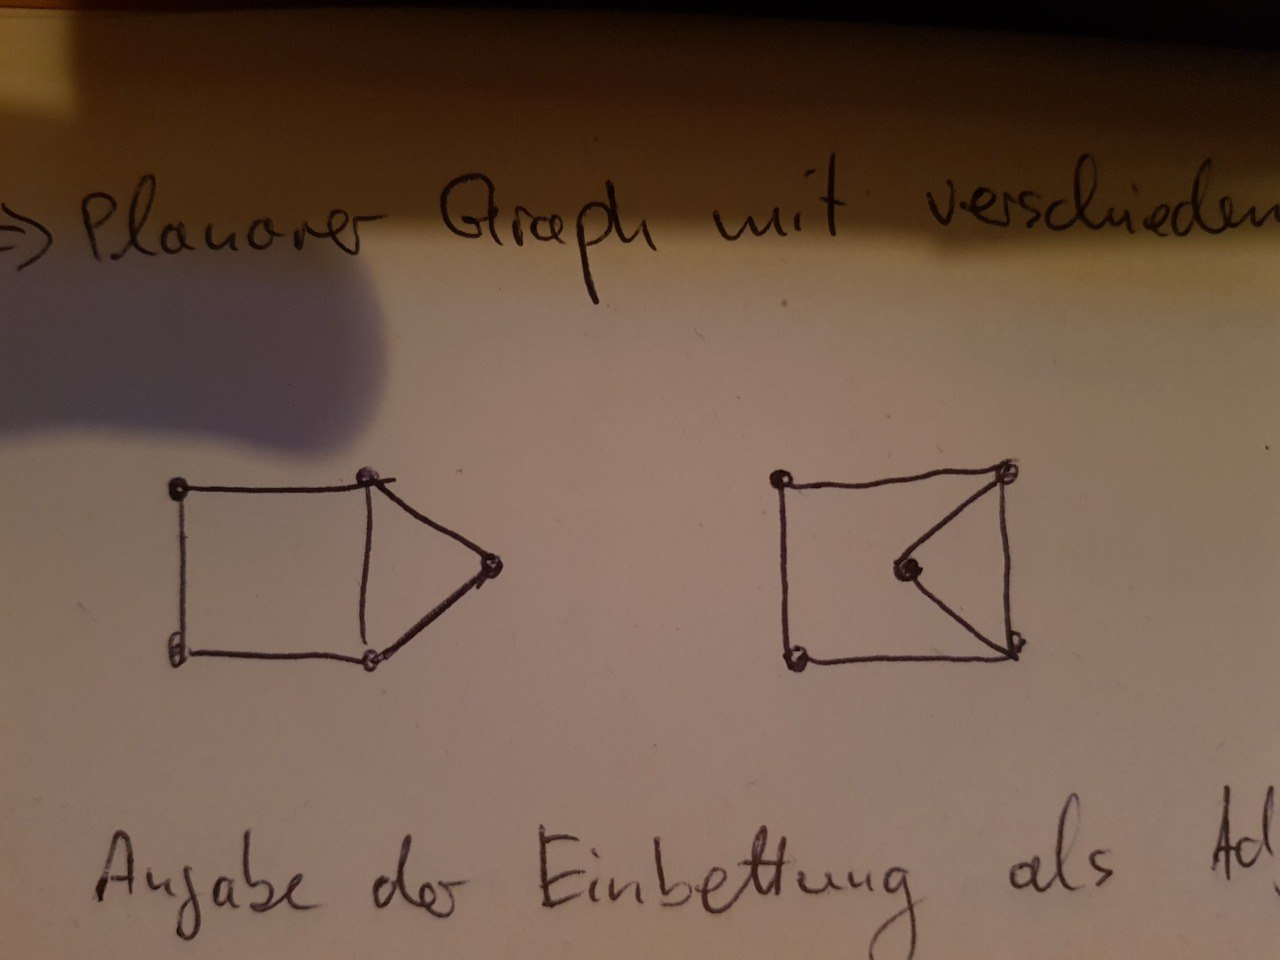
\includegraphics[width=10cm]{planar}
        \caption{Planarer Graph mit verschiedenen Einbettungen}
        \label{fig:}
    \end{center}
\end{figure}

Ein Graph hat eine eindeutige planare Einbettung, wenn er 3-fach zusammenhängend ist.
